\documentclass[10pt]{article}

\usepackage[margin=1in]{geometry}
\usepackage[T1]{fontenc}
\usepackage[utf8]{inputenc}
\usepackage{lmodern}
\usepackage{microtype}
\usepackage{booktabs}
\usepackage{float}
\usepackage{graphicx}
\usepackage{amsmath}
\usepackage{tikz}
\usetikzlibrary{arrows.meta,positioning}
\usepackage[font=footnotesize,labelfont=bf]{caption}
\usepackage[compact]{titlesec}
\titleformat{\section}{\large\bfseries}{\thesection}{0.6em}{}
\titlespacing*{\section}{0pt}{1.1ex plus 0.3ex}{0.5ex}
\usepackage[colorlinks=true,linkcolor=black,citecolor=black,urlcolor=blue]{hyperref}

\setlength{\parskip}{0.3em}
\setlength{\textfloatsep}{8pt plus 2pt minus 2pt}
\setlength{\floatsep}{6pt plus 2pt minus 2pt}
\setlength{\parindent}{0pt}
\renewcommand{\arraystretch}{1.0}
\setlength{\tabcolsep}{4.5pt}

\title{Few-Shot Reference Crops for Team and Goalkeeper Assignment\\in Football Broadcasts}
\author{J. Henrique Menezes\\Independent researcher\\\texttt{TODO}}
\date{}

\begin{document}
\maketitle

\begin{abstract}
Kit colours change every match, so a fixed classifier cannot assign football players to teams. We study a reference-conditioned formulation. Given the player boxes of a broadcast clip and $k$ labelled reference crops for each of four groups (team A, team B, goalkeeper A, goalkeeper B) taken earlier in the same half, a ResNet-18 embeds all crops and each box takes the group whose mean reference embedding is closest in cosine similarity. This is a prototypical network trained episodically; our contribution is the formulation, the evaluation and the comparison, not a new architecture. On 5,842 boxes from six held-out SoccerNet Game State Reconstruction matches, with identical ground-truth boxes, tracklets and pitch positions for both methods, the official SoccerNet baseline (PRTReID embeddings, per-clip K-means) scores 66.15\%, the mean of four per-group accuracies. Our model with six references and tracklet averaging scores 97.45\%. We also report reference-draw variance, rotated folds, a prospective replay, and Core ML latency (2.24 ms for 20 crops). Five SN-GSR-2025 clips have swapped outfield team labels; we give the evidence and use corrected labels.
\end{abstract}

\section{Introduction}

A broadcast analysis system must decide, for every player box, which team the player belongs to and whether the player is a goalkeeper. The answer cannot come from a fixed classifier, because kit colours change from match to match and goalkeepers wear kits that differ from both teams. The SoccerNet Game State Reconstruction (GSR) baseline~\cite{somers2024soccernet} handles this without labels. It embeds each box with PRTReID~\cite{mansourian2024prtreid}, clusters the embeddings of each clip into two groups with K-means, names each cluster by the mean pitch position of its members, and gives each goalkeeper the side of its own pitch position.

We ask a different question: how much does a small amount of labelled evidence from the same half help? An operator supplies $k$ labelled crops for each of four groups, taken earlier in the same half. A single four-way decision then assigns every box to team A, team B, goalkeeper A or goalkeeper B, and so ties each goalkeeper to a team. No clustering and no camera calibration are needed.

Methodologically, this is a prototypical network~\cite{snell2017prototypical} with a ResNet-18 encoder~\cite{he2016resnet}; we do not propose a new architecture. The contributions are the four-group formulation with references from the same half (Section~\ref{sec:method}); a like-for-like comparison with the official SoccerNet team method on 5,842 boxes from six held-out matches, with the same ground-truth tracklets and pitch coordinates for both (Section~\ref{sec:results}); an evaluation of reference choice, seeds, held-out matches, prospective use and box overlap (Sections~\ref{sec:variance}--\ref{sec:errors}); and the finding that five clips of SN-GSR-2025 have swapped outfield team labels (Section~\ref{sec:audit}). Code, checkpoints, results and the label audit are at \url{https://github.com/Hmenez3s/four-reference-team-classifier}.

\section{Related work}

\textbf{Game state reconstruction.} SoccerNet GSR~\cite{somers2024soccernet} defines the task of tracking and identifying athletes on a pitch minimap and provides the baseline described above. PRTReID~\cite{mansourian2024prtreid} is a multi-task model for re-identification, team affiliation and role classification; the baseline uses its role head (player, goalkeeper, referee, other) and its embeddings.

\textbf{Team discrimination without match-specific labels.} Istasse et al.~\cite{istasse2019associative} learn an embedding for game-agnostic team discrimination, and Koshkina et al.~\cite{koshkina2021contrastive} use contrastive learning for unsupervised player classification. Both aim to separate teams in a new match without labelled examples from that match. We use a few labelled crops from the target half instead, and we classify goalkeepers jointly with teams.

\textbf{Few-shot classification.} Prototypical networks~\cite{snell2017prototypical} classify a query by its distance to class prototypes, each the mean embedding of a few labelled support examples, and train the embedding on episodes that mimic the test situation. Our classifier uses this mechanism with cosine similarity. We also use a frozen re-identification network, OSNet~\cite{zhou2019osnet}, as a comparison encoder.

\section{Method}
\label{sec:method}

\begin{figure}[H]
\centering
\resizebox{\linewidth}{!}{%
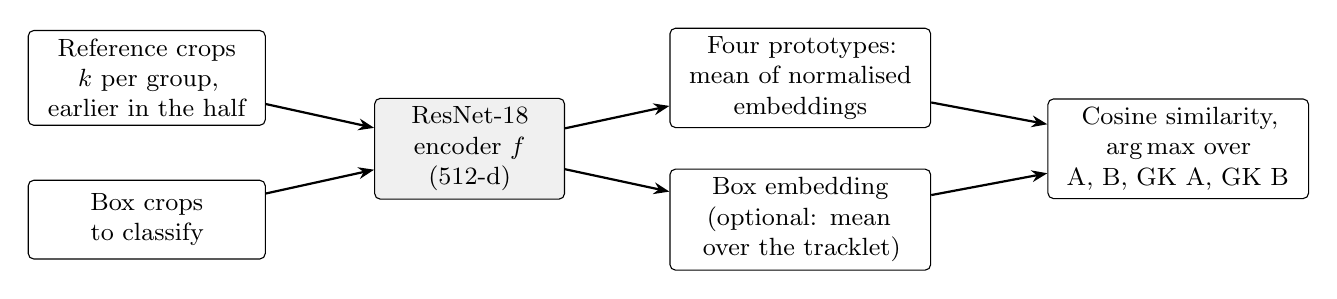
\begin{tikzpicture}[
  box/.style={draw, rounded corners=2pt, align=center, font=\small, minimum height=10mm, inner sep=3pt},
  arr/.style={-{Stealth[length=2mm]}, thick}]
  \node[box, text width=28mm] (ref) at (0,0.9) {Reference crops\\$k$ per group,\\earlier in the half};
  \node[box, text width=28mm] (qry) at (0,-0.9) {Box crops\\to classify};
  \node[box, text width=22mm, fill=black!6] (enc) at (4.1,0) {ResNet-18\\encoder $f$\\(512-d)};
  \node[box, text width=31mm] (pro) at (8.3,0.9) {Four prototypes:\\mean of normalised\\embeddings};
  \node[box, text width=31mm] (vec) at (8.3,-0.9) {Box embedding\\(optional: mean\\over the tracklet)};
  \node[box, text width=31mm] (out) at (13.1,0) {Cosine similarity,\\arg\,max over\\A, B, GK~A, GK~B};
  \draw[arr] (ref) -- (enc);
  \draw[arr] (qry) -- (enc);
  \draw[arr] (enc) -- (pro);
  \draw[arr] (enc) -- (vec);
  \draw[arr] (pro) -- (out);
  \draw[arr] (vec) -- (out);
\end{tikzpicture}}
\caption{Method. One encoder embeds the reference crops and the box crops. Each group prototype is the mean of its normalised reference embeddings, and each box takes the group with the highest cosine similarity.}
\label{fig:method}
\end{figure}

\textbf{Task.} The input is a set of player boxes, in the form of image crops, from one half of a match, plus $k$ labelled reference crops for each of four groups: team~A, team~B, goalkeeper~A and goalkeeper~B. Team~A is whichever team appears in the team-A references, so the same model works for any kit colours. Detection and tracking are outside the classifier. Referees receive one of the four labels, because there is no referee group.

\textbf{Model.} Each crop is resized to fit $96\times48$ pixels (height $\times$ width) with its aspect ratio preserved and is padded with black. A ResNet-18~\cite{he2016resnet} initialised with ImageNet weights~\cite{russakovsky2014imagenet} has its final fully connected layer removed, so the output is a 512-dimensional vector $f(x)$. Only \texttt{layer3} and \texttt{layer4} are fine-tuned; the other layers are frozen and batch normalisation stays in evaluation mode. For group $c$ with reference crops $x_{c,1},\dots,x_{c,k}$, the prototype is
\begin{equation}
p_c=\frac{1}{k}\sum_{i=1}^{k}\frac{f(x_{c,i})}{\lVert f(x_{c,i})\rVert},
\end{equation}
and a box $q$ is assigned to $\arg\max_c \cos\big(f(q),p_c\big)$. During training the logits are $20\cos(f(q),p_c)$ and the loss is cross-entropy.

\textbf{Tracklet averaging.} Optionally, the embeddings of all boxes of one tracklet in the half are averaged and normalised before the comparison, and the tracklet takes one label. The SoccerNet baseline also pools information per tracklet, so this gives both methods the same information. It needs tracklets and works offline over the half.

\textbf{Episodic training.} An episode samples one training half and draws one reference crop per group from its early part. For outfield groups the reference is an athlete, and queries exclude that athlete. Up to four box crops per group from the later part of the half serve as queries. For six references, five more crops of the same athlete (or goalkeeper) from other earlier frames are added to each group. We train for 8 epochs of 180 episodes with AdamW~\cite{loshchilov2017adamw} (learning rate $2\times10^{-4}$, weight decay $10^{-4}$) and cosine learning-rate decay. The checkpoint with the best macro recall on the validation matches is kept. We train two models: one with one reference per group and one with six.

\section{Experimental protocol}
\label{sec:protocol}

\textbf{Data.} SN-GSR-2025 has 164 clips from 18 match halves (9 matches). The matches are split into train (4, 6, 9), validation (2, 3, 5) and test (7, 8, 11) sets. For every half, references come from the part before a cutoff time, and the evaluated boxes come from the later part. In the retrospective protocol used for most results, the reference athlete is chosen so that it differs from the evaluated athletes, and later jersey labels are used to enforce this. These figures are therefore not deployment estimates. We use the corrected team labels of Section~\ref{sec:audit} throughout.

\textbf{Metric.} Goalkeepers are about 6\% of the boxes. Plain accuracy hides goalkeeper errors. We therefore report the \emph{score}, the mean of the four per-group accuracies (macro recall). Each goalkeeper group counts as much as each team. We also report plain accuracy, where every box counts once.

\textbf{Comparison with the SoccerNet method.} The baseline predicts a role and an embedding per box with PRTReID. Roles are majority-voted per tracklet. The mean embeddings of player tracklets are split by \texttt{KMeans(n\_clusters=2, random\_state=0)} per clip. Each cluster takes the side of its mean pitch position, and each goalkeeper takes the side of its own pitch position~\cite{sngamestate}. We ran this logic on the same boxes that we score, with ground-truth tracklets and pitch coordinates instead of a detector, a tracker and a camera calibration. This removes upstream errors for both methods. Boxes the baseline cannot assign (a non-player role or a missing pitch position) count as wrong. We also report two diagnostic variants: the baseline with true roles, and the baseline with true roles and, for each clip, the cluster-to-team mapping that is best according to the ground truth. The second is an oracle upper bound.

\textbf{Provenance.} The official PRTReID checkpoint~\cite{prtreid2024weights} was trained on SoccerNet-Tracking train, according to the PRTReID paper. Those 57 clips are exactly the SN-GSR-2025 train clips (matches 4, 6, 9), so no evaluated match was seen by it. Our models for matches 7, 8, 11 were trained on 4, 6, 9 and selected on 2, 3, 5. For matches 2, 3, 5, we retrained on 7, 8, 11 and selected on 4, 6, 9. The six evaluated matches contain 2,756, 2,761, 155 and 170 boxes in team~A, team~B, goalkeeper~A and goalkeeper~B, 5,842 in total.

\section{Comparison with the SoccerNet baseline}
\label{sec:results}

Table~\ref{tab:main} gives the pooled result on the six held-out matches. The baseline scores 66.15\%. Six references with tracklet averaging score 97.45\%. With each box classified alone, six references score 92.42\%, still above the baseline. The baseline is weakest on goalkeepers (57.42\% and 58.82\%).

\begin{table}[H]
\centering
\caption{Six held-out matches, 5,842 boxes. Score is the mean of the four per-group accuracies; accuracy counts every box once. GK is goalkeeper.}
\label{tab:main}
\small
\begin{tabular}{lrrrrrr}
\toprule
Method & Score & Accuracy & Team A & Team B & GK A & GK B \\
\midrule
SoccerNet baseline (PRTReID + K-means) & 66.15 & 73.30 & 71.84 & 76.53 & 57.42 & 58.82 \\
\quad with true roles & 92.79 & 88.38 & 84.07 & 91.56 & 96.13 & 99.41 \\
\quad with true roles, best mapping (oracle) & 94.00 & 90.65 & 86.28 & 94.17 & 96.13 & 99.41 \\
\midrule
Ours, 1 reference, each box & 87.69 & 91.00 & 89.84 & 92.97 & 83.23 & 84.71 \\
Ours, 1 reference, tracklets & 91.27 & 94.20 & 91.44 & 97.68 & 87.74 & 88.24 \\
Ours, 6 references, each box & 92.42 & 93.12 & 92.13 & 94.28 & 90.32 & 92.94 \\
Ours, 6 references, tracklets & \textbf{97.45} & \textbf{98.13} & 96.88 & 99.57 & 98.06 & 95.29 \\
\bottomrule
\end{tabular}
\end{table}

Table~\ref{tab:sets} splits the result by match set. On matches 7, 8, 11 its accuracy is 97.29\%, higher than ours with each box alone (96.77\%), but its score is 83.55\% because goalkeepers are assigned correctly in only 76.62\% and 59.26\% of boxes. On matches 2, 3, 5 its score is 50.93\%. In match 3 the baseline's role vote marks 418 of the 1,072 scored boxes as referees or the ball, and each of those counts as an error. With true roles, its score on matches 2, 3, 5 rises to 89.41\%, and the best cluster-to-team mapping gives the same score, so the remaining errors come from K-means splitting a team. On matches 7, 8, 11 the pitch-side rule also swaps teams in some clips: true roles give 96.65\%, and the best mapping gives 99.31\%. That oracle value is slightly above our 98.98\%. Over six matches, the oracle gives 94.00\%.

\begin{table}[H]
\centering
\caption{Score and accuracy per set of held-out matches. Matches 7, 8, 11: 2,659 boxes. Matches 2, 3, 5: 3,183 boxes.}
\label{tab:sets}
\small
\begin{tabular}{lrrrr}
\toprule
 & \multicolumn{2}{c}{Matches 7, 8, 11} & \multicolumn{2}{c}{Matches 2, 3, 5} \\
\cmidrule(lr){2-3}\cmidrule(lr){4-5}
Method & Score & Accuracy & Score & Accuracy \\
\midrule
SoccerNet baseline (official) & 83.55 & 97.29 & 50.93 & 53.25 \\
\quad with true roles, best mapping (oracle) & 99.31 & 99.25 & 89.41 & 83.47 \\
\midrule
Ours, 1 reference, each box & 86.10 & 95.60 & 89.49 & 87.15 \\
Ours, 1 reference, tracklets & 88.99 & 98.16 & 93.64 & 90.89 \\
Ours, 6 references, each box & 93.81 & 96.77 & 91.34 & 90.07 \\
Ours, 6 references, tracklets & \textbf{98.98} & \textbf{99.70} & \textbf{96.08} & \textbf{96.83} \\
\bottomrule
\end{tabular}
\end{table}

The comparison is not symmetric in what each method receives. The baseline uses no labelled crop from the evaluated half. Our method uses 24 labelled crops per half (four with one reference). Both sets of weights were trained on other matches.

\begin{figure}[H]
\centering
\begin{minipage}[c]{0.23\linewidth}
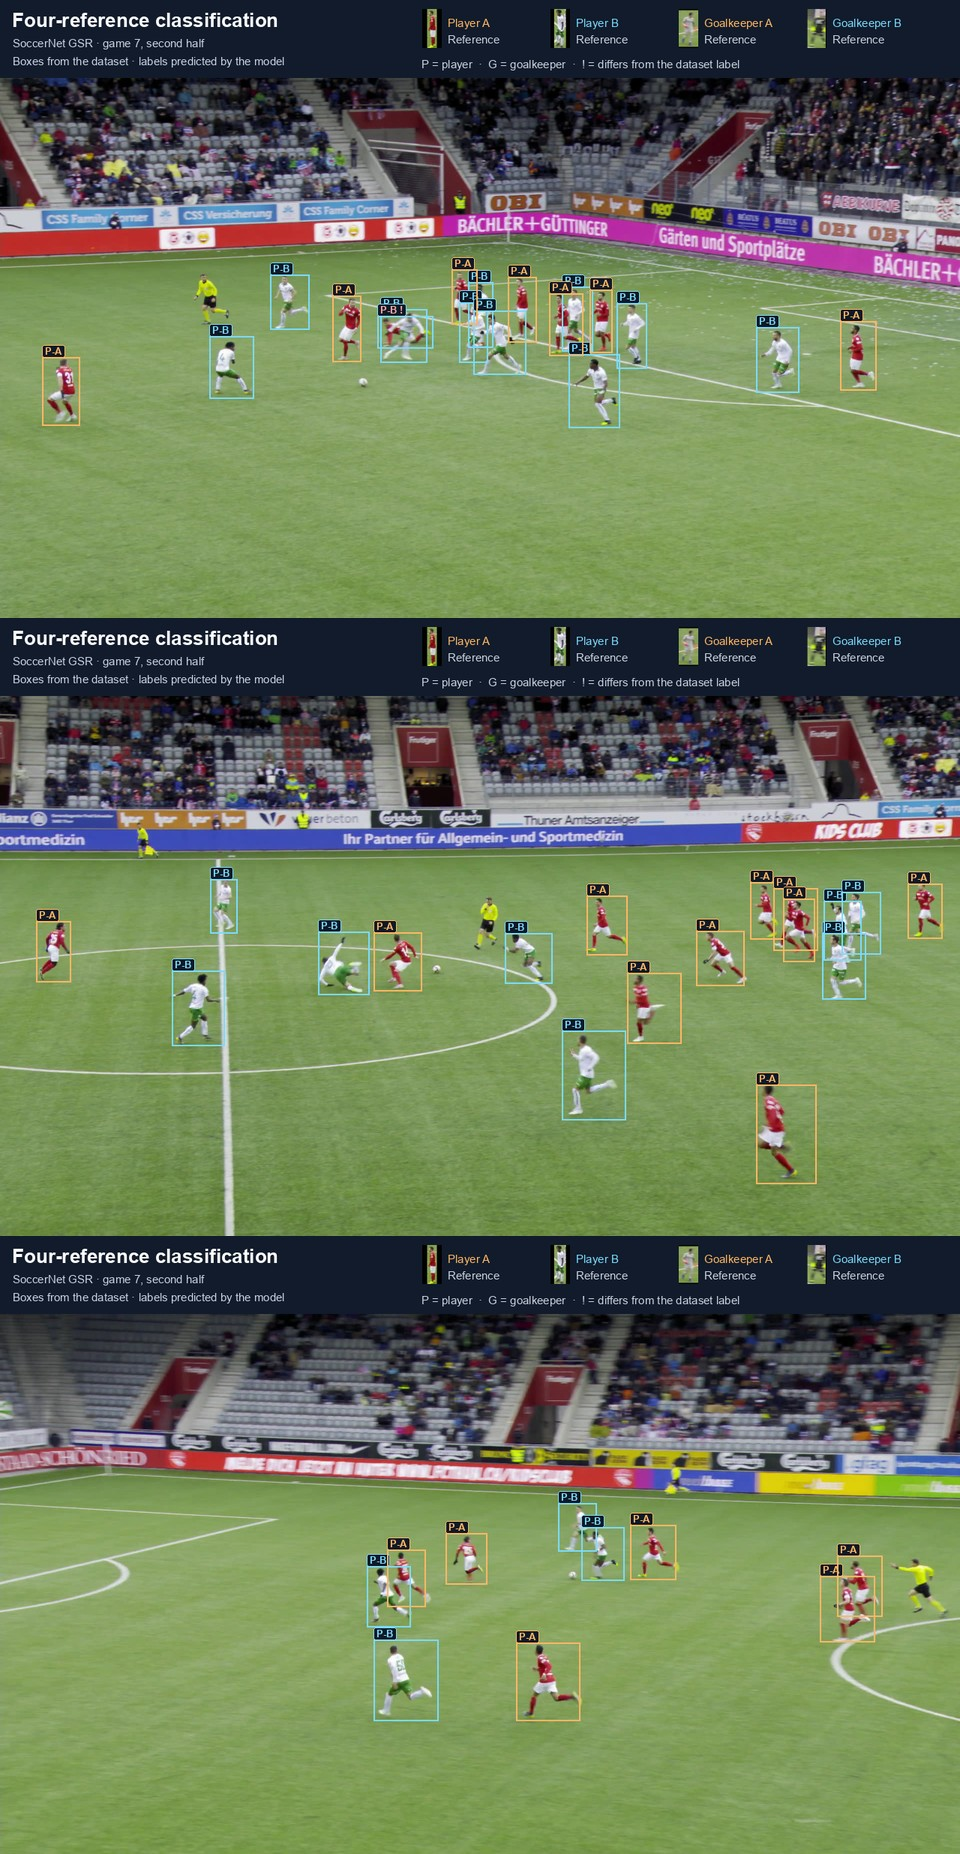
\includegraphics[width=\linewidth]{figures/classification-game-7-frames.jpg}
\end{minipage}\hfill
\begin{minipage}[c]{0.73\linewidth}
\caption{Three frames from the second half of match 7 (SoccerNet GSR), classified with one reference per group (the four crops at the top of each frame). Orange and blue boxes are the two teams. \texttt{P} is an outfield player and \texttt{G} a goalkeeper. \texttt{!} marks a label that differs from the dataset. On the 150-frame window from which the frames are taken (2,443 boxes), accuracy is 96.32\%. The window is illustrative and is not the test set.}
\label{fig:frames}
\end{minipage}
\end{figure}

\section{Reference choice, seeds and held-out matches}
\label{sec:variance}

\textbf{Effect of fine-tuning and of the number of references.} Table~\ref{tab:fixed} uses the fixed test split (matches 7, 8, 11; 2,659 boxes), with one fixed reference choice. A frozen ImageNet ResNet-18 with one reference scores 48.06\%. Fine-tuning for the task raises this to 86.10\% with one reference and 93.81\% with six. Goalkeepers gain most from additional references.

\begin{table}[H]
\centering
\caption{Fixed test split (matches 7, 8, 11), 2,659 boxes.}
\label{tab:fixed}
\small
\begin{tabular}{lrrrrrr}
\toprule
Model & Score & Accuracy & Team A & Team B & GK A & GK B \\
\midrule
ImageNet ResNet-18, not fine-tuned, 1 reference & 48.06 & 55.28 & 57.22 & 55.27 & 40.26 & 39.51 \\
Fine-tuned, 1 reference & 86.10 & 95.60 & 96.05 & 97.73 & 75.32 & 75.31 \\
Fine-tuned, 6 references & \textbf{93.81} & \textbf{96.77} & 96.45 & 97.89 & 88.31 & 92.59 \\
\bottomrule
\end{tabular}
\end{table}

\textbf{Thirty reference draws.} The fixed result depends on one choice of reference crops. We repeat the evaluation on the same test queries with 30 random reference choices per half. Each one-reference draw is nested in the corresponding six-reference draw, and for an outfield group the six crops show one athlete. Table~\ref{tab:draws} compares the fine-tuned models with three appearance baselines that use the same references: a frozen ImageNet ResNet-18, an HSV torso-colour descriptor, and a frozen Market-1501 OSNet~\cite{zhou2019osnet}. With six references the fine-tuned model trained with one reference scores 94.10\% $\pm$ 0.46, the colour descriptor 85.02\%, OSNet 80.72\% and the frozen ImageNet network 69.37\%. With one reference the same model scores 90.17\% $\pm$ 2.64: fewer references give a lower mean and a larger spread. The standard deviations are over reference choices on the same three matches, not over new matches.

\begin{table}[H]
\centering
\caption{Thirty paired reference draws on the fixed test queries (matches 7, 8, 11). Mean $\pm$ sample standard deviation, in percentage points. Score is the mean of the four per-group accuracies.}
\label{tab:draws}
\small
\begin{tabular}{lcccc}
\toprule
 & \multicolumn{2}{c}{Score} & \multicolumn{2}{c}{Accuracy} \\
\cmidrule(lr){2-3}\cmidrule(lr){4-5}
Encoder & 1 reference & 6 references & 1 reference & 6 references \\
\midrule
Fine-tuned, trained with 1 reference & 90.17 $\pm$ 2.64 & 94.10 $\pm$ 0.46 & 95.82 $\pm$ 1.28 & 97.15 $\pm$ 0.37 \\
Fine-tuned, trained with 6 references & 89.70 $\pm$ 2.41 & 93.58 $\pm$ 0.72 & 95.72 $\pm$ 1.04 & 96.78 $\pm$ 0.26 \\
HSV torso colour & 74.88 $\pm$ 4.52 & 85.02 $\pm$ 2.94 & 78.53 $\pm$ 5.70 & 85.24 $\pm$ 4.56 \\
Frozen Market-1501 OSNet & 61.88 $\pm$ 5.44 & 80.72 $\pm$ 3.22 & 60.63 $\pm$ 5.62 & 79.15 $\pm$ 3.82 \\
Frozen ImageNet ResNet-18 & 50.27 $\pm$ 4.34 & 69.37 $\pm$ 2.61 & 54.60 $\pm$ 5.96 & 72.30 $\pm$ 2.69 \\
\bottomrule
\end{tabular}
\end{table}

\textbf{Training seeds.} Five training seeds of the one-reference model on the same split give a score of 89.00\% $\pm$ 2.86 and an accuracy of 95.92\% $\pm$ 0.70.

\textbf{Rotated folds.} Three folds hold out whole matches in turn (7, 8, 11; 2, 3, 5; 4, 6, 9), with the one-reference model. Fold scores are 86.10\%, 89.49\% and 80.53\%, and fold accuracies are 95.60\%, 87.15\% and 85.77\%. Pooled over the nine matches (9,130 boxes), the score is 85.04\% and the accuracy 89.11\%. These folds are internal to SN-GSR-2025 and do not test another dataset.

\section{Prospective replay}
\label{sec:prospective}

The retrospective protocol uses later jersey labels to choose references. To check how this affects the result, we replay a prospective protocol. References come from the first 30\% of the labelled timestamps of a half, and up to 192 uniformly sampled frames of that period are considered. Queries are all valid boxes in up to 96 uniformly sampled later frames. Later boxes are not filtered by jersey.

Coverage is partial. Both arms cover \textbf{3 of the 6} test halves (match 7 half 2, match 8 halves 1 and 2). In the other three halves, the early period has no usable labelled crop for at least one goalkeeper group. We score the same 3,688 later boxes in the three covered halves. With the model trained with one reference, accuracy is 96.29\% with one early reference per group and 97.02\% with six. With the model trained with six references, it is 94.69\% and 95.47\%. This is not a coverage rate for other matches. The query population differs from that of the retrospective protocol, so accuracies are not comparable across the two.



\section{Error analysis by box overlap}
\label{sec:errors}

On the fixed one-reference test, 117 of 2,659 boxes are wrong. We group boxes by the largest intersection with another annotated person box, divided by the area of the box. This is a proxy for overlap, not a measure of physical occlusion or of the cause of an error. The error rate rises with overlap: 3.11\% (53 of 1,704 boxes) with no overlap, 3.77\% for overlap in $[0.1,0.3)$, 8.98\% in $[0.3,0.6)$, and 21.09\% (27 of 128 boxes) at 0.6 or more. Of the 53 errors with no overlap, 47 cross the boundary between outfield player and goalkeeper.



\section{Swapped team labels in SN-GSR-2025}
\label{sec:audit}

In SN-GSR-2025, the \texttt{team} attribute is \texttt{left} or \texttt{right} relative to the camera, so it carries no team identity across clips by itself. Within one match half, the labels should agree between clips. We compared the jersey numbers of the outfield players under each label across all clips of the same half. In 5 of the 164 clips, the jersey numbers under each label appear in the other clips mostly under the opposite label (Table~\ref{tab:audit}). In these clips the outfield \texttt{team} labels are swapped; the goalkeeper labels are consistent with the rest of the half. The clips are SNGS-092 (validation), SNGS-111 (train) and SNGS-126, SNGS-131 and SNGS-197 (test).

Figure~\ref{fig:swap} shows an example. In the reference clip SNGS-128, white-and-green outfield players are labelled \texttt{right} and red players \texttt{left}. In the flagged clip SNGS-131 it is the reverse, and the jersey numbers agree with this reading (for example \#4, \#27 and \#50 in white and green, and \#9 and \#31 in red; numbers worn by both teams are ignored). The goalkeeper under \texttt{left} in SNGS-131 has a median pitch position of $-48.6$, at the opposite end from the keeper under \texttt{right} in SNGS-128 ($35.8$), so the goalkeeper labels were not swapped. We reported the finding and a fix upstream (\url{https://github.com/SoccerNet/sn-gamestate/issues/39}). The fix swaps \texttt{left} and \texttt{right} for the outfield players of each flagged clip and leaves goalkeepers unchanged. Our preprocessing applies it, and every result in this paper uses the corrected labels, including the SoccerNet baseline.

\begin{figure}[H]
\centering
\begin{minipage}[t]{0.47\linewidth}
\vspace{0pt}
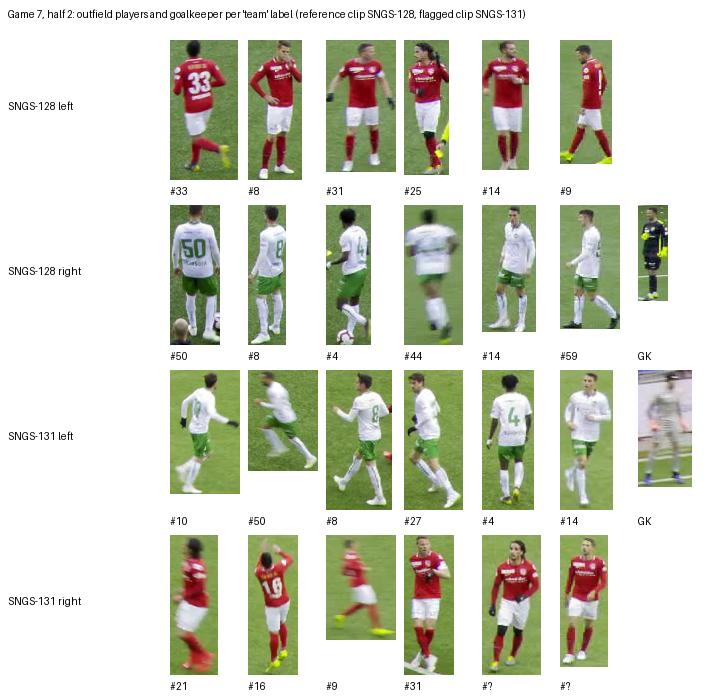
\includegraphics[width=\linewidth]{figures/SNGS-131.jpg}
\captionof{figure}{Match 7, half 2. Outfield players (with jersey number) and a goalkeeper (GK) under each \texttt{team} label, for the reference clip SNGS-128 and the flagged clip SNGS-131. White-and-green players are under \texttt{right} in SNGS-128 and under \texttt{left} in SNGS-131. Red players are the other way around.}
\label{fig:swap}
\end{minipage}\hfill
\begin{minipage}[t]{0.50\linewidth}
\vspace{0pt}
\captionof{table}{Clips with swapped outfield team labels. Counts are the clip's jersey numbers found in other clips of the same half under the same or opposite label.}
\label{tab:audit}
\footnotesize
\setlength{\tabcolsep}{3pt}
\begin{tabular}{llcrr}
\toprule
Clip & Split & Match, half & Same & Opposite \\
\midrule
SNGS-092 & validation & 5, 2 & 3 & 125 \\
SNGS-111 & train & 6, 2 & 4 & 68 \\
SNGS-126 & test & 7, 2 & 10 & 39 \\
SNGS-131 & test & 7, 2 & 10 & 34 \\
SNGS-197 & test & 11, 2 & 3 & 49 \\
\bottomrule
\end{tabular}
\end{minipage}
\end{figure}

\section{Deployment}
\label{sec:deployment}

We measured the six-reference model on an Apple M4 Pro with batches of 20 prepared crops (Table~\ref{tab:deploy}), excluding decoding, detection and tracking. Core ML INT8 quantises weights and activations, with calibration crops only from training matches 4, 6, 9. On the Neural Engine, INT8 takes 2.24 ms for 20 crops and scores 93.79\%, against 93.81\% for PyTorch FP32 on the GPU.

\begin{table}[H]
\centering
\caption{Six-reference model on the fixed test split (2,659 boxes), Apple M4 Pro. Latency is the median per batch of 20 crops.}
\label{tab:deploy}
\small
\begin{tabular}{llrrr}
\toprule
Runtime & Precision & Score & Accuracy & Latency (ms) \\
\midrule
PyTorch GPU & FP32 & 93.81 & 96.77 & 6.17 \\
Core ML GPU & INT8 & 93.81 & 96.73 & 2.99 \\
Core ML Neural Engine & INT8 & 93.79 & 96.69 & \textbf{2.24} \\
\bottomrule
\end{tabular}
\end{table}

\section{Limitations}

All results use ground-truth boxes and tracklets, so detector and tracker errors are not measured. Six matches from one dataset were evaluated, and the nine-match folds are internal to it; we make no claim about other datasets. The method needs labelled crops of each group from the same half (24 with six references), and the prospective replay covered only 3 of 6 halves because goalkeeper references were missing in the others. The retrospective protocol uses later jersey labels to pick references, so its figures are not deployment estimates. The classifier has four classes, so a referee receives a team or goalkeeper label. The baseline was used with its published weights.

\bibliographystyle{plain}
\bibliography{references}

\end{document}
